\documentclass[tikz,border=12pt]{standalone}
\usepackage{amsmath,amssymb}
\usetikzlibrary{positioning,arrows,shapes,fit,calc,decorations.pathmorphing,backgrounds}
\begin{document}
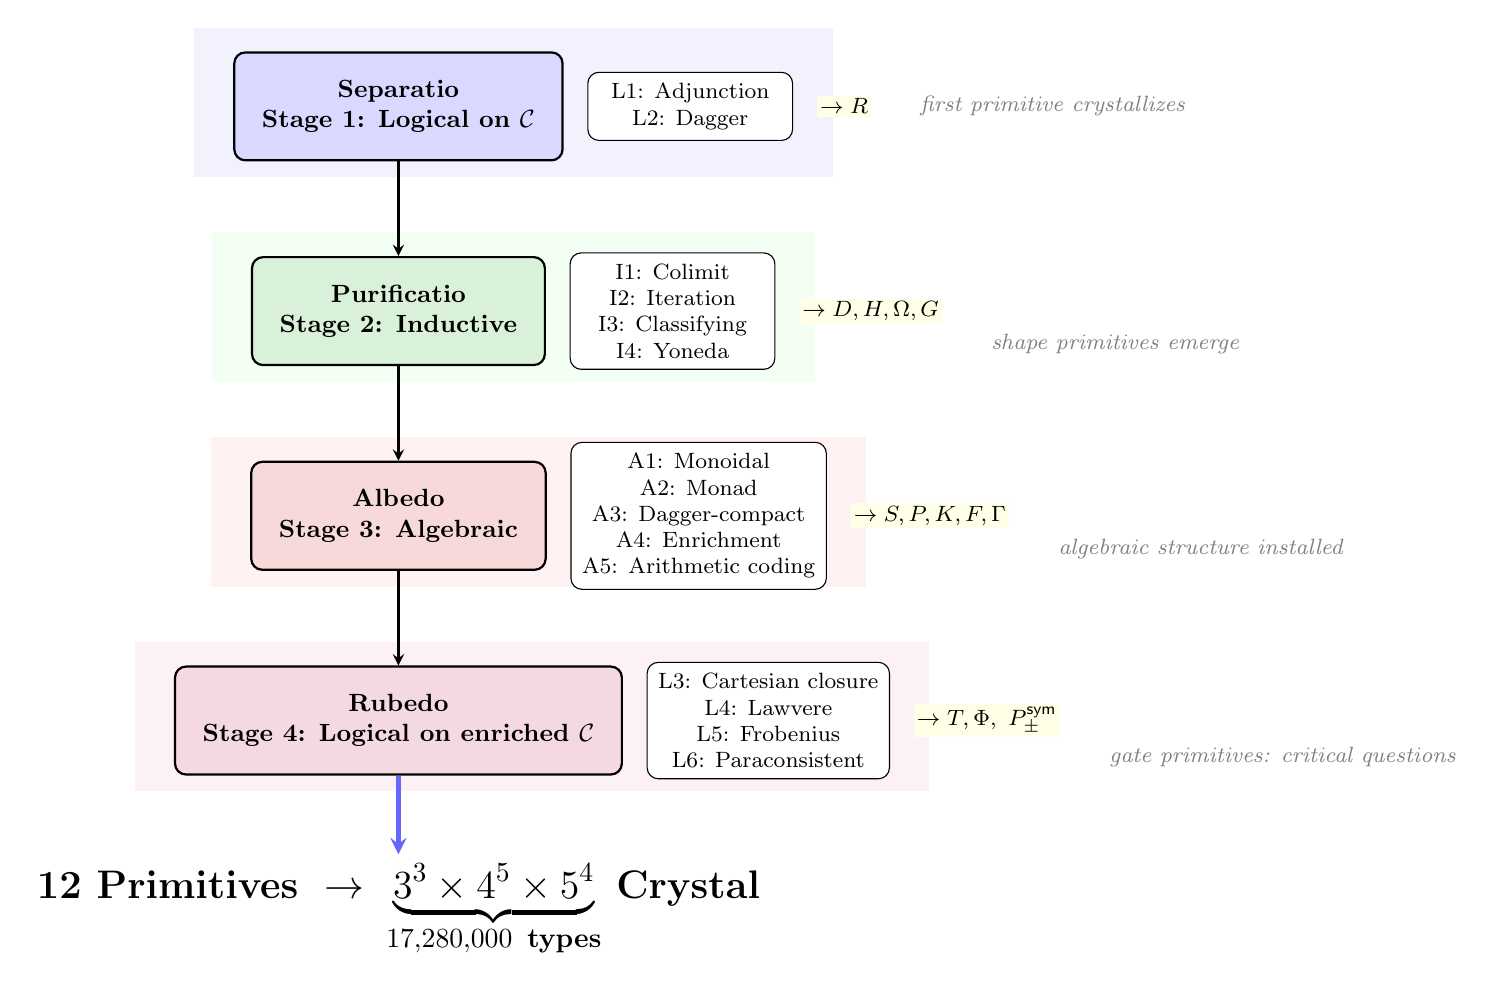
\begin{tikzpicture}[
  stage/.style={rectangle,draw,thick,rounded corners,fill=#1!15,inner sep=10pt,align=center,minimum width=2.8cm,font=\small\bfseries},
  ops/.style={rectangle,draw,fill=white,rounded corners,inner sep=4pt,font=\footnotesize,align=center,minimum width=2.6cm},
  arr/.style={->,>=stealth,thick},
  bigarr/.style={->,>=stealth,ultra thick,blue!60},
  prim/.style={font=\footnotesize\sffamily,fill=yellow!10,inner sep=1pt},
]

% Stage labels
\node[stage=blue]   (S1) at (0,0)     {\textsc{Separatio}\\Stage 1: Logical on $\mathcal{C}$};
\node[stage=green!60!black] (S2) at (0,-2.6) {\textsc{Purificatio}\\Stage 2: Inductive};
\node[stage=red!80!black]   (S3) at (0,-5.2) {\textsc{Albedo}\\Stage 3: Algebraic};
\node[stage=purple] (S4) at (0,-7.8) {\textsc{Rubedo}\\Stage 4: Logical on enriched $\mathcal{C}$};

% Arrows between stages
\draw[arr] (S1) -- (S2);
\draw[arr] (S2) -- (S3);
\draw[arr] (S3) -- (S4);

% Operations at each stage
\node[ops,right=0.3cm of S1] (ops1) {L1: Adjunction\\L2: Dagger};
\node[ops,right=0.3cm of S2] (ops2) {I1: Colimit\\I2: Iteration\\I3: Classifying\\I4: Yoneda};
\node[ops,right=0.3cm of S3] (ops3) {A1: Monoidal\\A2: Monad\\A3: Dagger-compact\\A4: Enrichment\\A5: Arithmetic coding};
\node[ops,right=0.3cm of S4] (ops4) {L3: Cartesian closure\\L4: Lawvere\\L5: Frobenius\\L6: Paraconsistent};

% Primitives at each stage
\node[prim,right=0.3cm of ops1] (p1) {$\to R$};
\node[prim,right=0.3cm of ops2] (p2) {$\to D, H, \Omega, G$};
\node[prim,right=0.3cm of ops3] (p3) {$\to S, P, K, F, \Gamma$};
\node[prim,right=0.3cm of ops4] (p4) {$\to T, \Phi,\ P_{\pm}^{\text{sym}}$};

% Final product
\node[below=1.0cm of S4,font=\Large\bfseries] (result) {12 Primitives $\;\to\; \underbrace{3^3 \times 4^5 \times 5^4}_{17{,}280{,}000\ \text{types}}$ Crystal};
\draw[bigarr] (S4) -- (result);

% Background bands
\begin{scope}[on background layer]
\fill[blue!5]  ($(S1.north west)+(-0.5,0.3)$) rectangle ($(ops1.south east|-S1.south)+(0.5,-0.2)$);
\fill[green!5] ($(S2.north west)+(-0.5,0.3)$) rectangle ($(ops2.south east|-S2.south)+(0.5,-0.2)$);
\fill[red!5]   ($(S3.north west)+(-0.5,0.3)$) rectangle ($(ops3.south east|-S3.south)+(0.5,-0.2)$);
\fill[purple!5]($(S4.north west)+(-0.5,0.3)$) rectangle ($(ops4.south east|-S4.south)+(0.5,-0.2)$);
\end{scope}

% Stage annotations
\node[font=\footnotesize\itshape,text=gray,right=0.5cm of p1,anchor=west] {first primitive crystallizes};
\node[font=\footnotesize\itshape,text=gray,right=0.5cm of p2.south east,anchor=north west] {shape primitives emerge};
\node[font=\footnotesize\itshape,text=gray,right=0.5cm of p3.south east,anchor=north west] {algebraic structure installed};
\node[font=\footnotesize\itshape,text=gray,right=0.5cm of p4.south east,anchor=north west] {gate primitives: critical questions};

\end{tikzpicture}
\end{document}
